\documentclass{article}

\usepackage{graphicx}
\usepackage{float}
\usepackage{amsmath, amssymb}
\title {Propuesta de aplicación para la planificación de evaluaciones}
\author{Juan Miguel Pérez Martínez, Amanda Noris Hernández , Marcos Antonio Pérez Lorenzo}
\begin{document}
\begin{titlepage}
\centering
{\bfseries\LARGE Universidad de La Habana \par}
\vspace{1cm}
{\scshape\Large Facultad de Matemática y Ciencias de la Computación \par}
\vspace{3cm}
{\scshape\Huge Creaci\'on de propuesta de aplicaci\'on y módulo de optimizaci\'on para la realizaci\'on de calendarios de ex\'amenes  \par}
\vspace{3cm}
{\itshape\Large Proyecto de la asignatura Modelos Matem\'aticos Aplicados\par}
\vfill
{\Large  Juan Miguel P\'erez Martínez  \\
Marcos Antonio Pérez Lorenzo  \\
Amanda Noris Hernández\par}

\vfill
{\Large Abril 2024 \par}
\end{titlepage}
\section{Introducción al problema}

\subsection{Contexto del Proyecto}

El proyecto se inició en respuesta a un problema recurrente en la facultad: la planificación de las evaluaciones de cada asignatura a lo largo del semestre. Este desafío se presenta cada semestre, poniendo en riesgo la eficiencia y la satisfacción de los estudiantes y profesores. La necesidad de encontrar una solución eficiente y efectiva para este problema es imperativa, ya que afecta directamente la calidad de la educación y la experiencia de aprendizaje de los estudiantes.
\subsection{Sobre el problema :}

En el ámbito académico, la planificación de evaluaciones es una tarea crítica que afecta directamente la eficiencia del proceso educativo y la satisfacción de los estudiantes y profesores. Este problema se presenta anualmente en muchas instituciones educativas, donde se requiere una solución que permita optimizar la distribución de las evaluaciones a lo largo del semestre, considerando los requisitos específicos de cada asignatura, las implicaciones para los estudiantes y la medición del impacto de estas decisiones en la experiencia de aprendizaje.

La necesidad de una solución eficiente y efectiva para este problema es imperativa, dado que una planificación adecuada de las evaluaciones puede mejorar significativamente la calidad de la educación, facilitar la gestión del tiempo de los estudiantes y profesores, y reducir los conflictos de horarios. Este informe presenta un enfoque innovador para abordar este problema, utilizando técnicas avanzadas de optimización y modelado matemático para diseñar una aplicación que permita determinar la mejor manera posible de planificar las evaluaciones, teniendo en cuenta todos los factores relevantes.
\section{Objetivo del Proyecto}

El objetivo principal de este proyecto es diseñar e implementar una aplicación que permita determinar la mejor manera posible de planificar las evaluaciones de cada asignatura a lo largo del semestre. Para lograr este objetivo, se considerarán varios factores clave:

\begin{enumerate}
\item Requisitos de las Asignaturas: Se analizarán las necesidades específicas de cada asignatura en términos de la cantidad de evaluaciones y el período ideal para realizarlas.
\item Conveniencia de las Evaluaciones: Se evaluará qué evaluaciones tiene sentido realizar en una misma semana, considerando la carga de trabajo para los estudiantes.
\item Implicaciones para los Estudiantes: Se medirá el impacto que tiene para los estudiantes la planificación de cada evaluación en una semana específica.
\end{enumerate}

\section{Metas y Objetivos Específicos}

Para alcanzar el objetivo principal del proyecto, se buscan los siguientes metas y objetivos específicos:

\begin{enumerate}
\item Análisis de Requisitos: Se buscará la manera de obtener los requisitos de cada asignatura, incluyendo la cantidad de evaluaciones y el período ideal para su realización.
\item Evaluación de Conveniencia: Identificar qué evaluaciones son convenientes realizar en una misma semana, teniendo en cuenta la carga de trabajo para los estudiantes.
\item Diseño de la Aplicación: Diseñar una aplicación que permita a los usuarios (profesores y estudiantes) planificar las evaluaciones de manera eficiente, considerando los requisitos de las asignaturas y el impacto para los estudiantes.
\item Feedback y Mejora Continua: Recopilar feedback de los usuarios y realizar mejoras continuas en la aplicación para optimizar la planificación de las evaluaciones.
\end{enumerate}
\section{Resultados Claves del Proyecto}
\begin{enumerate}
\item{Desarrollo de una Aplicación Web para la Gestión de Calendarios de Exámenes: }
La aplicación web desarrollada facilita la recopilación de datos necesarios para la planificación de calendarios de exámenes, permitiendo a los usuarios ingresar información relevante como fechas de exámenes, cursos, y asignaturas, así como la carga de trabajo que representa cada asignatura para cada uno.

\item{Implementación de un Algoritmo Genético para la Optimización de Calendarios :}
Se ha implementado un algoritmo genético que utiliza técnicas de cruce, mutación, y selección para optimizar la planificación de calendarios de exámenes. Este algoritmo busca minimizar conflictos de horarios y la carga de trabajo de los estudiantes, asegurando que todos los estudiantes puedan cumplir con sus obligaciones académicas.

\item{Mejora en la Eficiencia y Coherencia de los Calendarios de Exámenes :}
Gracias a la aplicación web y al algoritmo genético, se ha logrado una mejora significativa en la eficiencia y coherencia de los calendarios de exámenes.


\end{enumerate}

\section{Intentos de Optimización que no funcionaron}

\subsection{Optimización con pulp}
El primer intento se realizó utilizando la biblioteca pulp, que permite modelar problemas de optimización como problemas de programación lineal. Este enfoque tampoco funcionó por la linealidad. El código correspondiente se puede encontrar en el Anexo B.

\subsection{Optimización con scipy.optimize}
El segundo intento de optimización se realizó utilizando la función minimize de scipy.optimize, junto con NonlinearConstraint para definir restricciones específicas. Este enfoque no funcionó debido a la linealidad. El código correspondiente se puede encontrar en el Anexo A.

\subsection{Optimización con gurobipy}
El tercer intento se realizó utilizando gurobipy, una interfaz de Python para el solver Gurobi. Tampoco funcionó (no se implement\'o en su totalidad). El código correspondiente se puede encontrar en el Anexo C.

\subsection{Optimización con scipy.optimize y Clases Personalizadas}
El último intento se realizó utilizando scipy.optimize junto con clases personalizadas para definir el problema de optimización y el proceso de optimización. Este enfoque permitió una mayor flexibilidad y control sobre el proceso de optimización, incluyendo la capacidad de dividir el problema en subproblemas más pequeños y manejar de manera más eficiente las restricciones y la función objetivo. Aunque tampoco con esto pudimos lograr el objetivo. El código correspondiente se puede encontrar en el Anexo D.
\section{Definición del Modelo de Optimización}

Minimizar $f(x)$ donde $f: \mathbb{M}^{n \times m}(\mathbb{N}) \rightarrow \mathbb{R}$.

\begin{itemize}
\item $F$ es el conjunto de días no elegibles (días festivos, fines de semana, días no disponibles para el profesor o alumnos, etc.).
\item $V_{ij}$ es el conjunto de conjuntos de días elegibles para la j-ésima asignatura en el i-ésimo curso.
\item $k_{ij}$ es la carga de trabajo específica para la asignatura j-ésima del i-ésimo curso.
\item $D_i$ son los días totales correspondientes al curso i-ésimo.
\end{itemize}

La función objetivo $f(x)$ se define como:

\[
f(x) = \sum_{i=1}^{n} (ke_i + kp_i + kc_i)
\]

$$\text{s.a.}$$:
$$x_{ij}\notin F$$
$$x_{ij} \geq V_{ij0}$$
$$x_{ij} \leq V_{ij1}$$

donde:

\begin{itemize}
\item $E_{ijk}$ es un conjunto auxiliar para $ke_i$, definido como:

\[
E_{ijk} = 
\begin{cases} 
1 & \text{si } x_{ij} > k \\
0 & \text{en otro caso}
\end{cases}
\]

\item $C_{ik}$ es un conjunto auxiliar para $kc_i$, definido como:

\[
C_{ik} = 
\begin{cases} 
k_{ia} + k_{ib} & \text{si existe } a, b : X_{ia} = X_{ib} = k \\
0 & \text{en otro caso}
\end{cases}
\]

\item $ke_i$ es la carga del estudiante, calculada como:

\[
ke_i = \sum_{j=1}^{m} \sum_{k=1}^{D_i} E_{ijk} \cdot \frac{k_{ij}}{1 + |X_{ij} - V_{ij0}|}
\]

\item $kp_i$ es la carga de proximidad, calculada como:

\[
kp_i = \sum_{a=1}^{m} \sum_{b=1}^{m} \frac{k_{ia} + k_{ib}}{1 + |X_{ia} - X_{ib}|}
\]

\item $kc_i$ es la carga de trabajo específica, calculada como:

\[
kc_i = \sum_{k=1}^{D_i} C_{ik}
\]

\end{itemize}
\section{Algoritmo Genético para la Optimización de un Calendario de Exámenes}

El algoritmo genético es una técnica de optimización inspirada en la evolución natural, diseñada para encontrar soluciones óptimas o cercanas a óptimas a problemas complejos que son difíciles de resolver mediante métodos convencionales. Este enfoque se basa en la creación y evolución de una población de soluciones candidatas, cada una representada por una cadena de símbolos llamada cromosoma. Los cromosomas codifican los valores de las variables que definen el espacio de soluciones. La calidad de cada solución se mide mediante una función de aptitud, que asigna una puntuación numérica basada en qué tan bien la solución satisface los objetivos y restricciones del problema.

\subsection{Definición de la Función Objetivo y Restricciones}

El modelo de optimización se centra en minimizar una función objetivo que incluye cargas del estudiante, carga de proximidad y carga de trabajo específica. Las restricciones se refieren a los días elegibles para cada asignatura en cada curso. Este enfoque permite una representación precisa de los problemas de programación y horario, donde la calidad de una solución se evalúa en función de cómo se distribuyen los horarios de las asignaturas, teniendo en cuenta las restricciones de disponibilidad y preferencias.

\subsection{Representación de la Solución}

Cada solución en el algoritmo genético se representa como una cadena de bits, donde cada bit corresponde a un día elegible o no elegible para una asignatura en un curso. Esta representación permite una manipulación eficiente de las soluciones a través de operaciones genéticas como el cruce y la mutación. La función \texttt{decode} convierte esta cadena de bits en una representación numérica que puede ser evaluada por la función objetivo, facilitando así la evaluación de la calidad de las soluciones candidatas.

\subsection{Operaciones Genéticas}

\subsubsection{Cruce (cross)}

Se realiza un cruce entre dos soluciones seleccionadas, combinando partes de ambas soluciones para generar nuevas soluciones. Este proceso introduce diversidad en la población y ayuda a explorar diferentes combinaciones de horarios.

\subsubsection{Mutación (mutate)}

Se realiza una mutación en una solución, cambiando aleatoriamente algunos de los bits. Esto introduce variación en la población y ayuda a evitar quedar atrapado en óptimos locales.

\subsubsection{Selección (selection)}

Se seleccionan soluciones para el próximo ciclo de cruce y mutación basándose en sus puntuaciones. Las soluciones con mejores puntuaciones tienen más probabilidades de ser seleccionadas, lo que favorece la evolución hacia soluciones de mayor calidad.

\subsection{Optimización}

La función \texttt{optimize} implementa el algoritmo genético, inicializando una población de soluciones y realizando iteraciones de cruce, mutación y selección para mejorar la solución. La mejor solución encontrada se devuelve al final, proporcionando una solución óptima o cercana a óptima para el problema de programación de horarios.

\subsection{Integración con el Problema Específico}

Para adaptar el algoritmo genético al problema de optimización descrito, se definen la función objetivo y las restricciones en el contexto de este problema. Esto se hace en la clase \texttt{Problem}, donde se definen las funciones \texttt{kc}, \texttt{ke}, y \texttt{kp} para calcular las cargas de trabajo específicas, la carga de proximidad y la carga de trabajo específica, y la función \texttt{f} para la función objetivo. Esta integración permite que el algoritmo genético se aplique directamente al problema específico de optimización de horarios, utilizando las restricciones y objetivos definidos para guiar la búsqueda de soluciones óptimas.

\subsection{Ejecución del Algoritmo}

Finalmente, se ejecuta el algoritmo genético llamando al método \texttt{optimize} de la clase \texttt{Problem}, pasando los parámetros necesarios como el número de intentos, tamaño de la población y número de generaciones. Este proceso permite la evolución de la población de soluciones a lo largo de varias generaciones, mejorando continuamente la calidad de las soluciones candidatas hasta que se alcanza una solución óptima o se cumplen los criterios de terminación. 

\section{Propuesta de Aplicación para la Optimización de Calendarios de Exámenes}

En esta sección, presentamos una propuesta de aplicación diseñada para mejorar la gestión y optimización de los calendarios de exámenes en instituciones educativas. La aplicación se centra en la autenticación de usuarios y en la asignación de diferentes niveles de acceso permitiendo una gestión eficiente y segura de los calendarios de exámenes.

\subsection{Autenticación de Usuarios}

La aplicación implementa un sistema de autenticación  que permite a los usuarios acceder a la plataforma de manera segura. Una vez autenticados, los usuarios tienen la capacidad de cambiar sus contraseñas, lo que asegura la seguridad de sus cuentas. Este sistema de autenticación es esencial para garantizar que solo los usuarios autorizados puedan acceder a la información y realizar cambios en los calendarios de exámenes.

\begin{figure}[h!] \centering 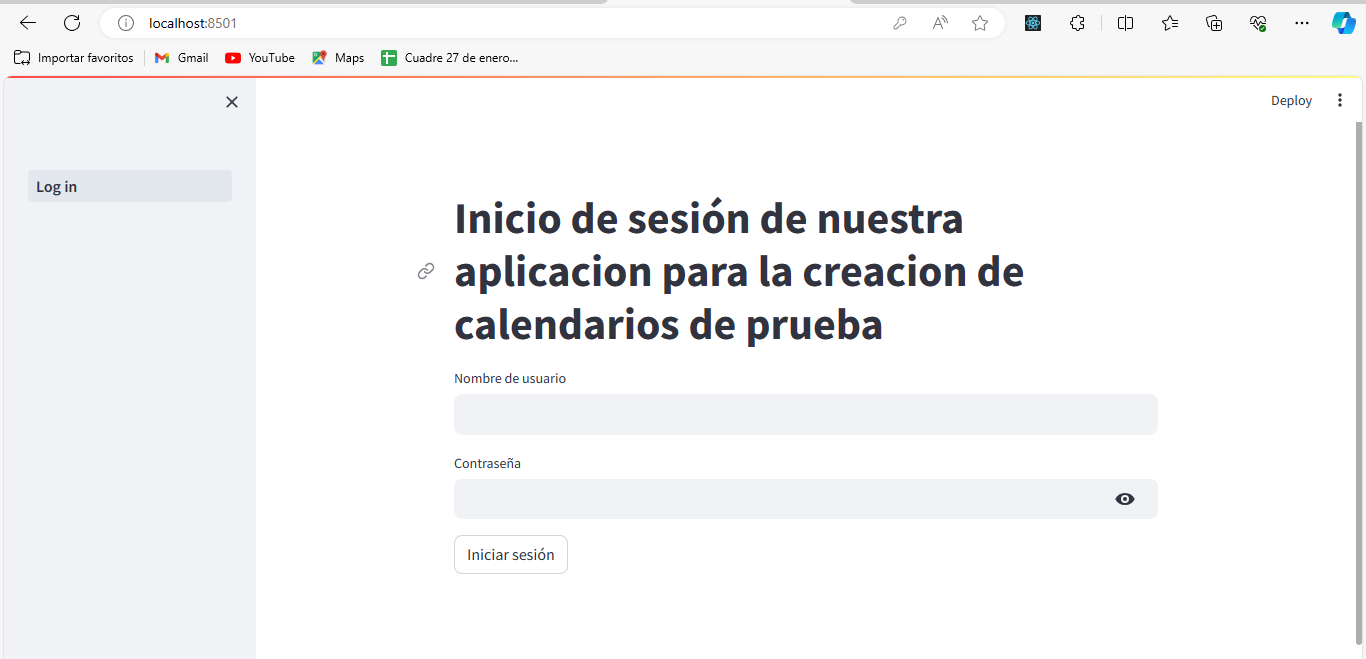
\includegraphics[width=0.5\textwidth]{autenticacion_usuario.png} \caption{Pantalla de autenticación de usuario.} \end{figure}

\subsection{Niveles de Acceso}

La aplicación define tres niveles de acceso distintos, cada uno con un conjunto específico de funcionalidades:

\subsubsection{Usuario}

El nivel de acceso de usuario permite a los usuarios calificar asignaturas en términos de carga de trabajo y visualizar los calendarios de exámenes. Esta funcionalidad es crucial para que los estudiantes puedan evaluar la carga de trabajo de sus asignaturas y planificar adecuadamente su tiempo.

\begin{figure}[h!] \centering 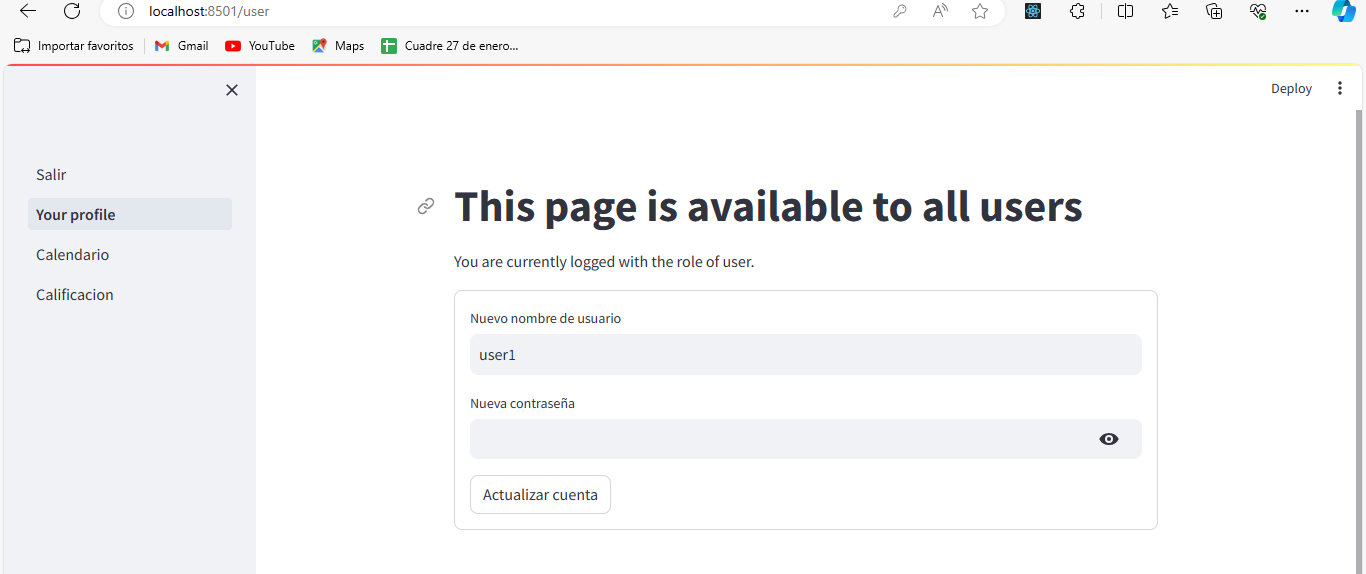
\includegraphics[width=0.5\textwidth]{nivel_usuario.png} \caption{Funcionalidades del nivel de acceso de usuario.} \end{figure}

\subsubsection{Administrador}

El nivel de acceso de administrador amplía las capacidades del usuario, permitiendo la adición de nuevos usuarios a la aplicación y la inclusión de asignaturas en el calendario. Este nivel de acceso es vital para la gestión de la plataforma, ya que permite a los administradores mantener actualizada la información relevante para los estudiantes y profesores.

\begin{figure}[h!] \centering 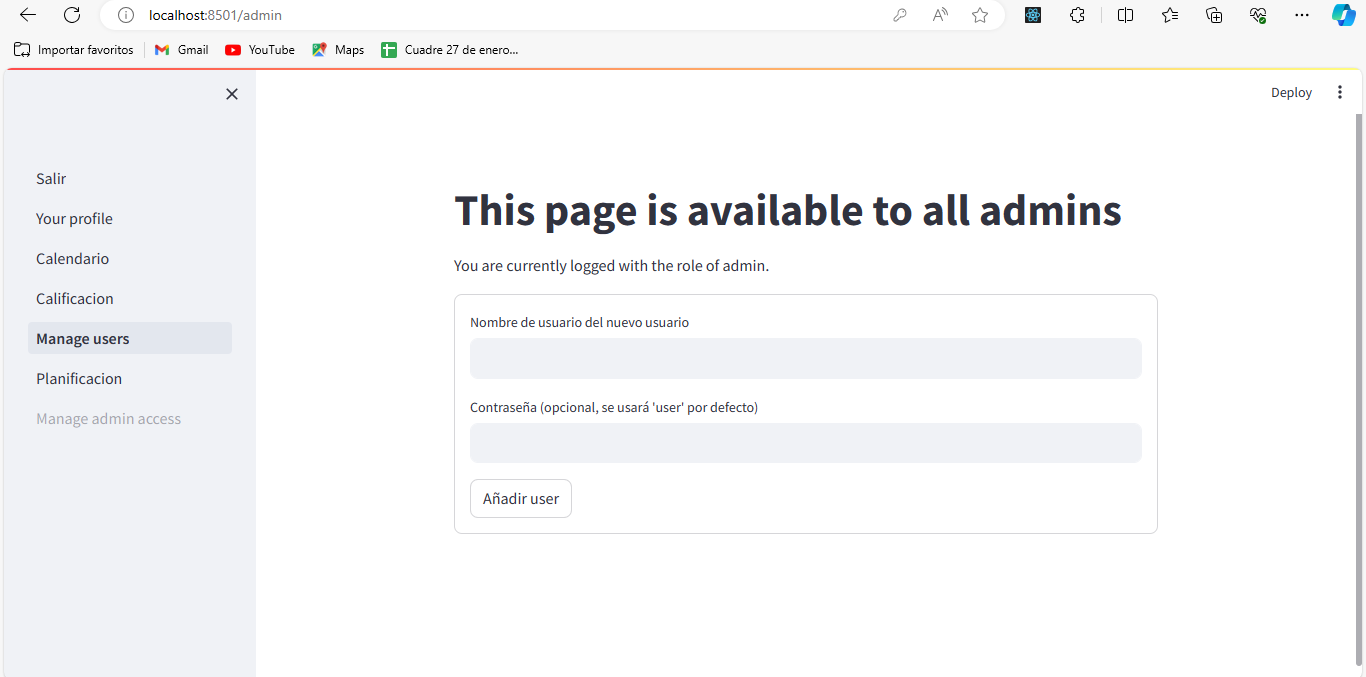
\includegraphics[width=0.5\textwidth]{nivel_administrador.png} \caption{Funcionalidades del nivel de acceso de administrador.} \end{figure}

\subsubsection{Superadmin}

El nivel de acceso de superadmin es el más alto, otorgando todas las funcionalidades disponibles en la aplicación. Los superadmins tienen la capacidad de ejecutar el módulo de optimización para crear el calendario de exámenes de todos los cursos. Este nivel de acceso es esencial para la toma de decisiones estratégicas y la implementación de cambios a gran escala en la gestión de los calendarios de exámenes.

\begin{figure}[h!] \centering 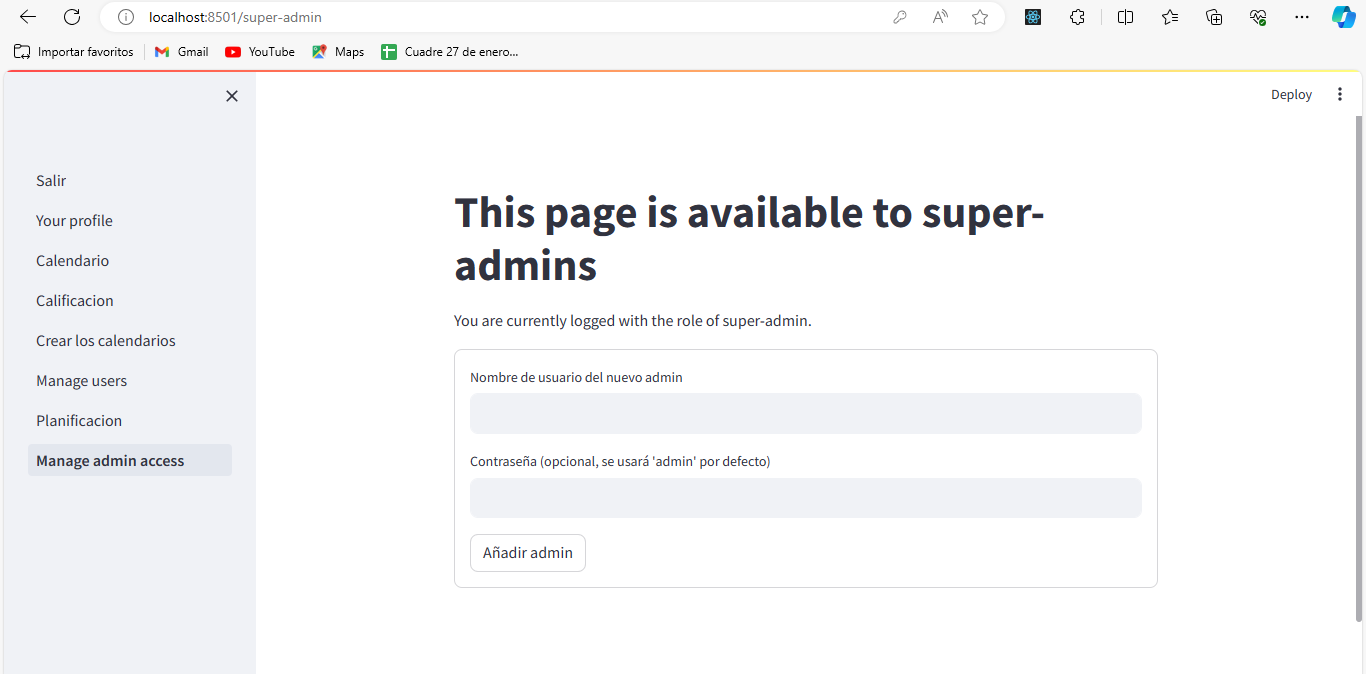
\includegraphics[width=0.5\textwidth]{nivel_superadmin.png} \caption{Funcionalidades del nivel de acceso de superadmin.} \end{figure}
\subsection{Funcionalidad de Salir}

La funcionalidad de salir permite a los usuarios cerrar sesión de manera segura. Esta funcionalidad es esencial para garantizar la privacidad y seguridad de los datos del usuario.

\begin{figure}[h!] \centering 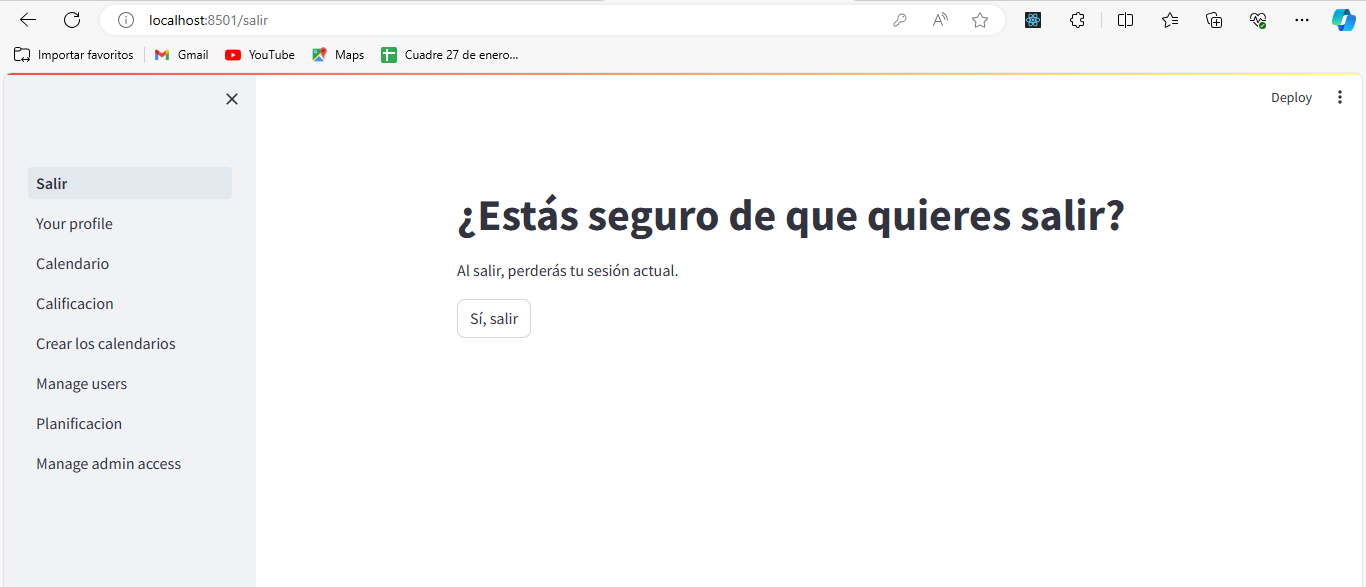
\includegraphics[width=0.5\textwidth]{salir.png} \caption{Pantalla de salir.} \end{figure}

\subsection{Funcionalidad de Perfil de Usuario}

El perfil de usuario permite a los usuarios ver y editar su contraseña y en una versión futura todo lo relacionado con su  información personal. Esta funcionalidad es crucial para mantener actualizada la información del usuario y facilitar la personalización de la experiencia de usuario.

\begin{figure}[h!] \centering 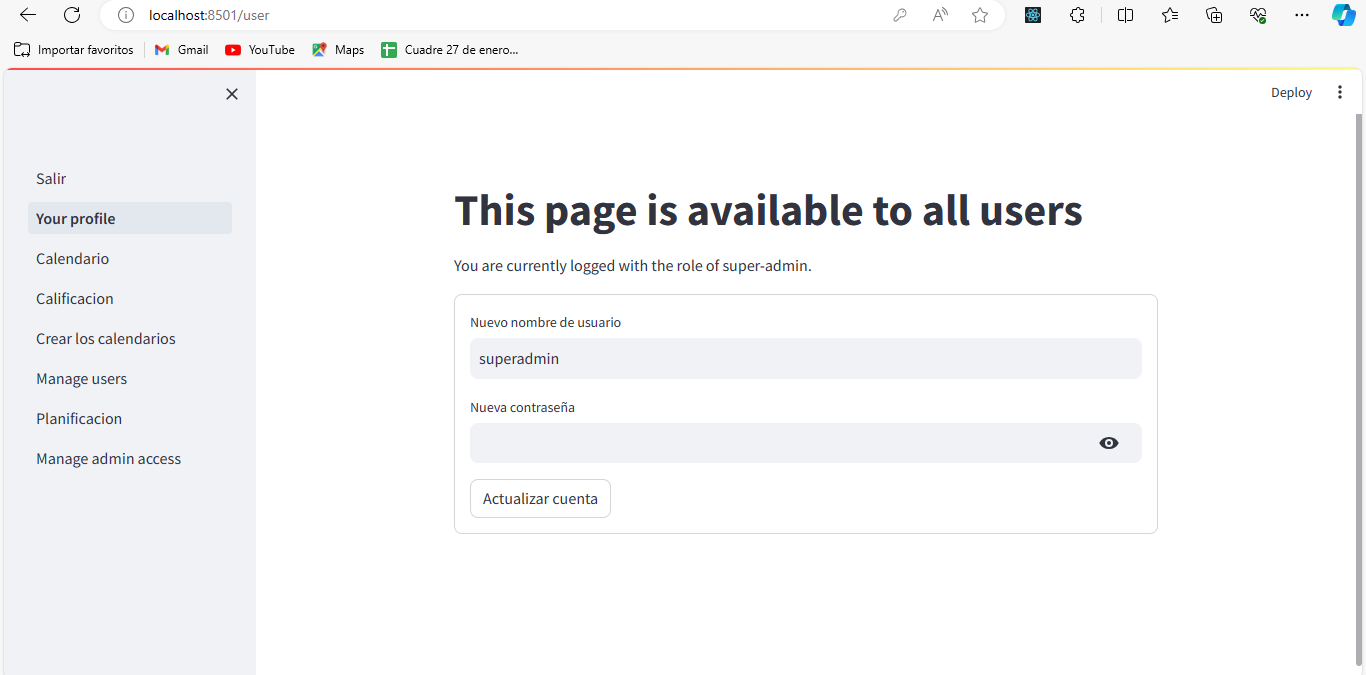
\includegraphics[width=0.5\textwidth]{perfil_usuario.png} \caption{Pantalla de perfil de usuario.} \end{figure}

\subsection{Funcionalidad de Calendario}

El calendario permite a los usuarios visualizar sus horarios de exámenes . Esta funcionalidad es esencial para la planificación y gestión del tiempo de los estudiantes.

\begin{figure}[H] \centering 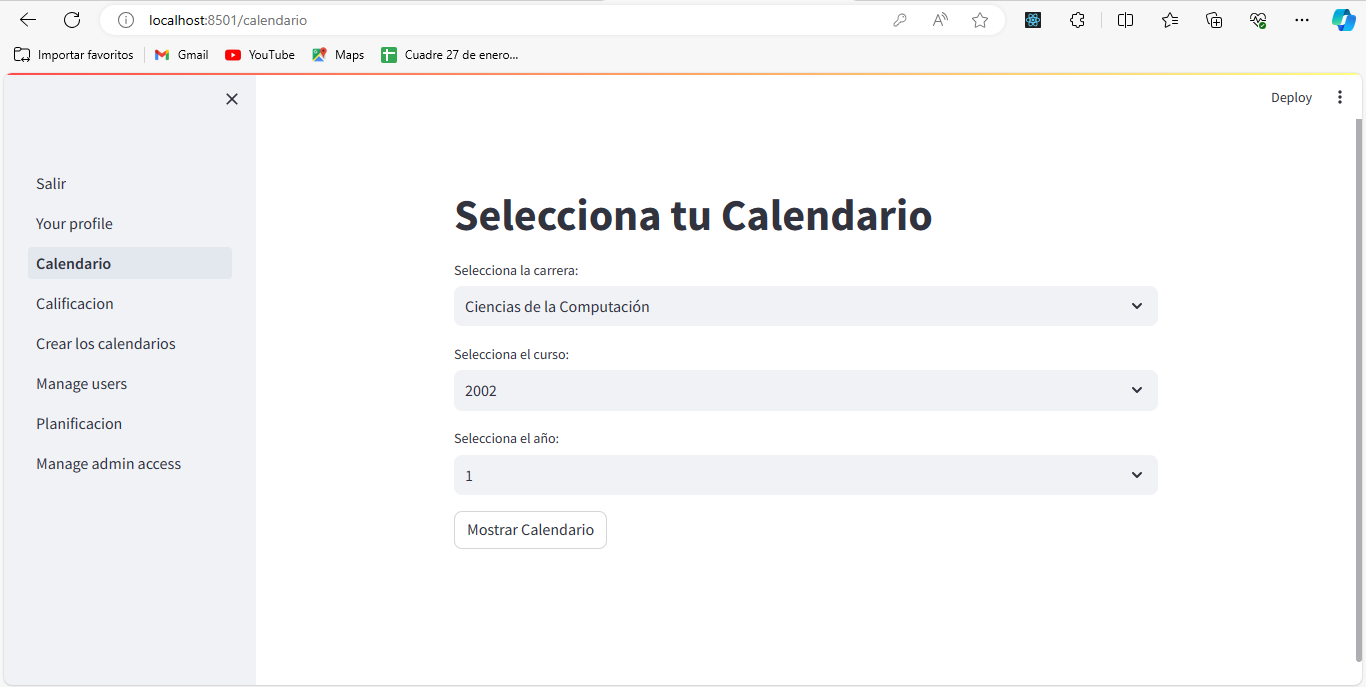
\includegraphics[width=0.5\textwidth]{calendario.png} \caption{Pantalla del calendario.} \end{figure}

\begin{figure}[h!] \centering 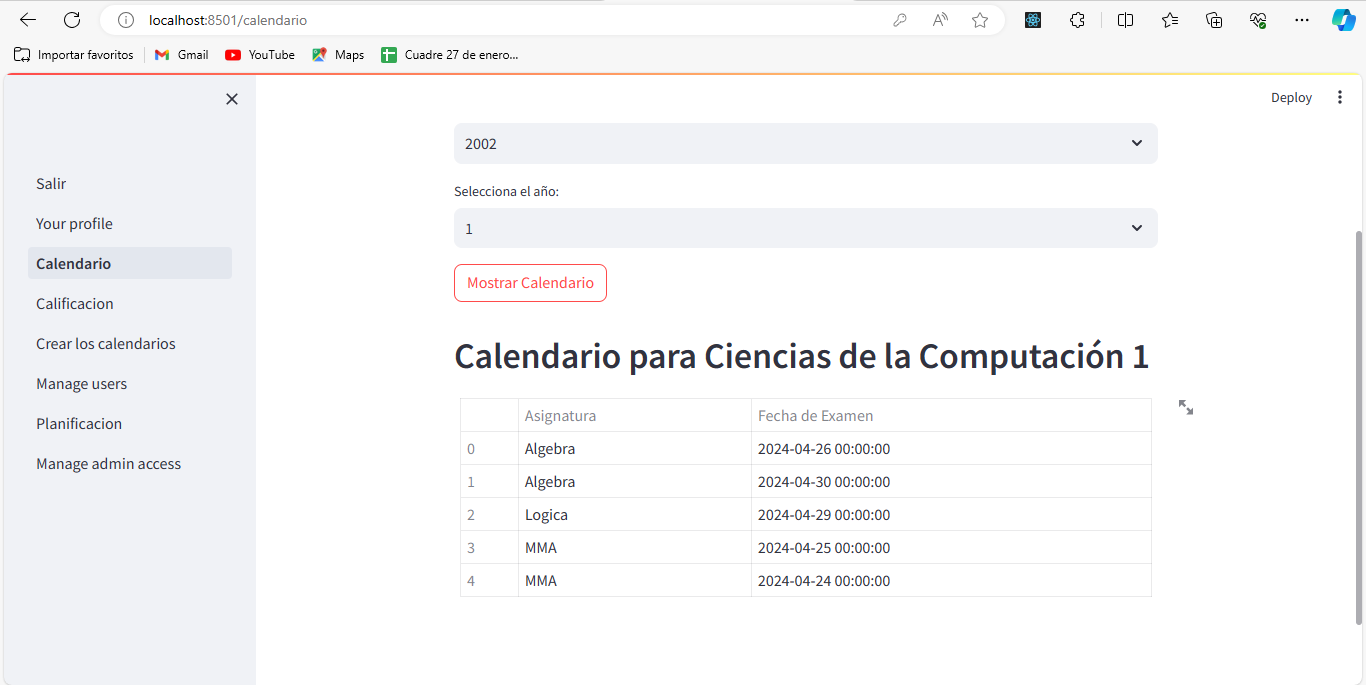
\includegraphics[width=0.5\textwidth]{calendario1.png} \caption{Pantalla del calendario.} \end{figure}

\subsection{Funcionalidad de Calificación}

La funcionalidad de calificación permite a los usuarios calificar asignaturas en términos de carga de trabajo. Esta funcionalidad es crucial para evaluar la carga de trabajo de las asignaturas y planificar adecuadamente el tiempo.

\begin{figure}[h!] \centering 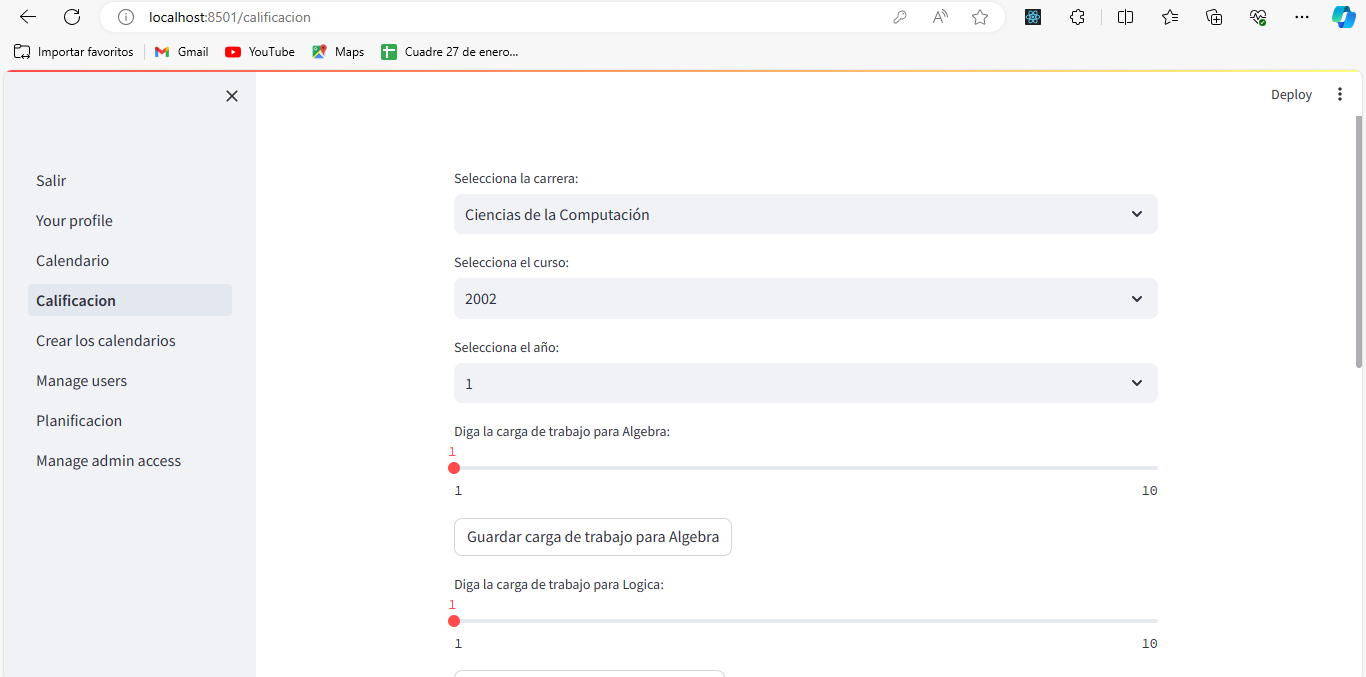
\includegraphics[width=0.5\textwidth]{calificacion.png} \caption{Pantalla de calificación.} \end{figure}

\subsection{Funcionalidad de Crear Calendarios}

La funcionalidad de crear calendarios permite a los superadmins  generar calendarios de exámenes para todos los cursos. Esta funcionalidad es esencial para la gestión y optimización de los horarios de exámenes, aquí es donde se ejecuta el módulo de optimización.

\begin{figure}[H] \centering 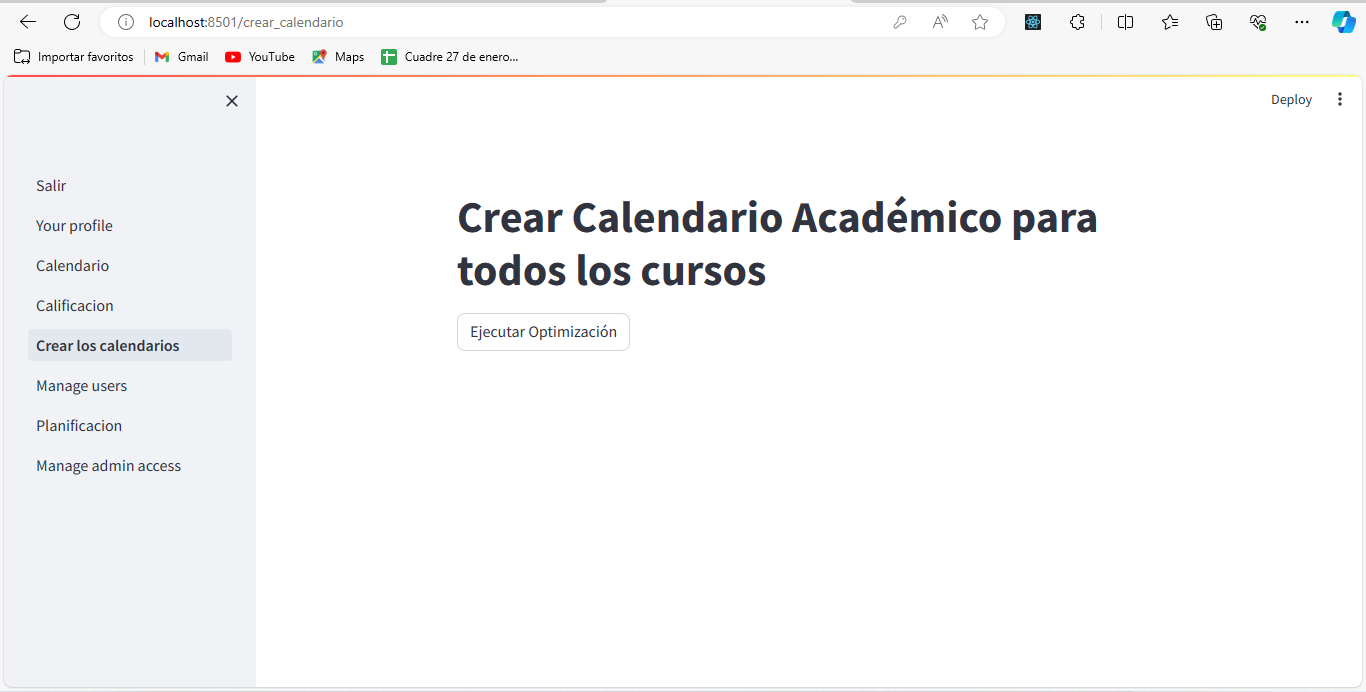
\includegraphics[width=0.5\textwidth]{crear_calendarios.png} \caption{Pantalla de creación de calendarios.} \end{figure}

\subsection{Funcionalidad de Gestión de Usuarios}

La gestión de usuarios permite a los administradores y superadmins añadirusuarios en un futuro si se quisiera sería sencillo poner la funcionalidad de  editar y eliminar usuarios. Esta funcionalidad es vital para la administración de la plataforma.

\begin{figure}[H] \centering 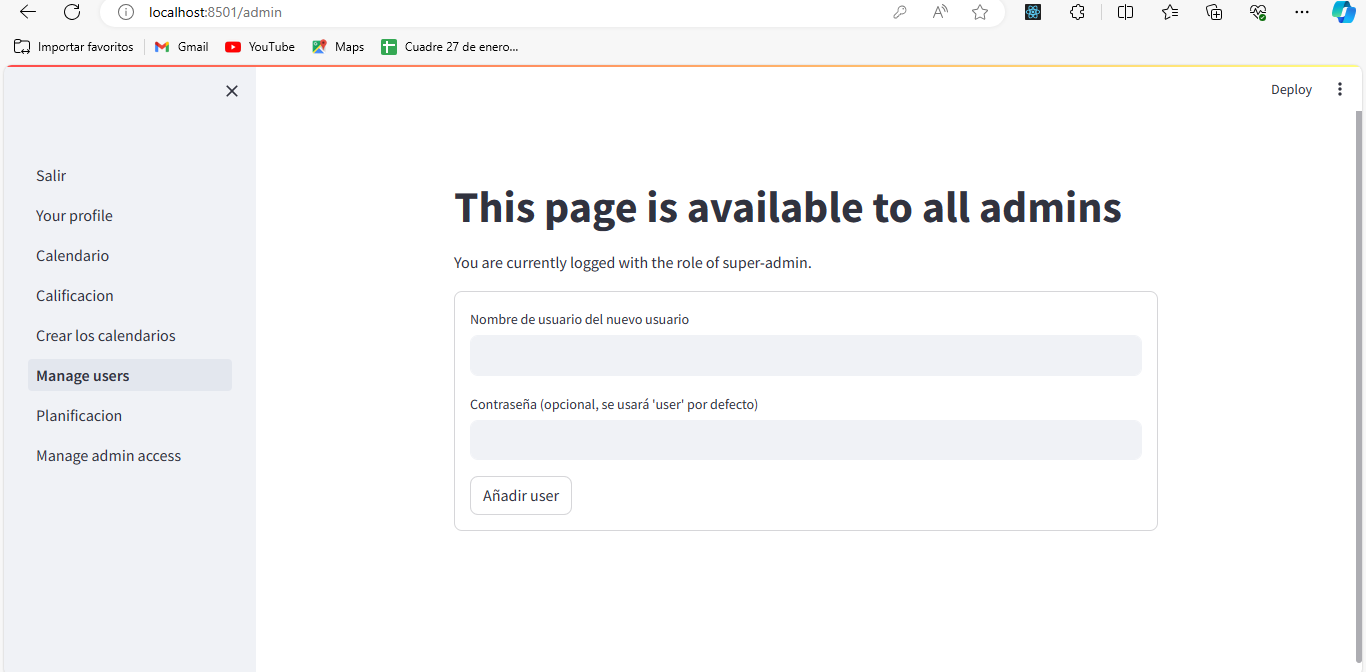
\includegraphics[width=0.5\textwidth]{gestion_usuarios.png} \caption{Pantalla de gestión de usuarios.} \end{figure}

\subsection{Funcionalidad de Planificación}

La funcionalidad de planificación permite a los administradores y superadmins planificar asignaturas y exámenes. Esta funcionalidad es crucial para la organización y distribución de los horarios de exámenes.

\begin{figure}[h!] \centering 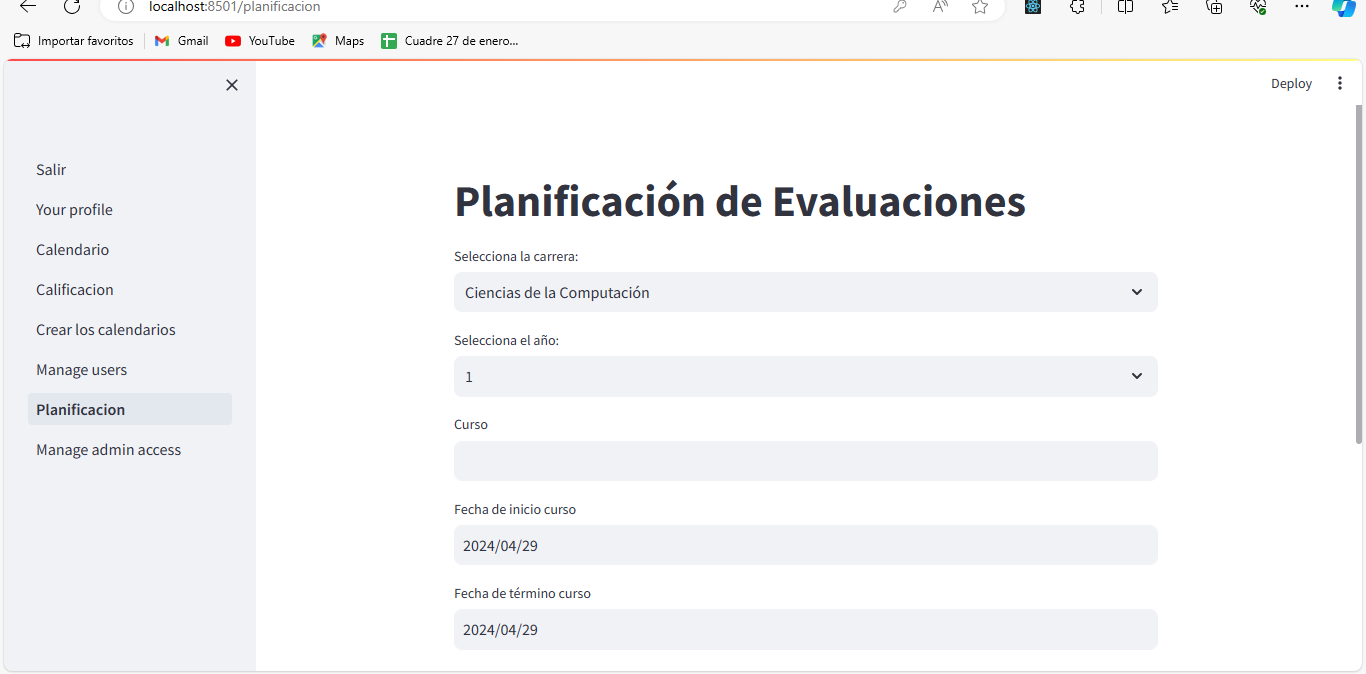
\includegraphics[width=0.5\textwidth]{planificacion.png} \caption{Pantalla de planificación.} \end{figure}

\subsection{Funcionalidad de Gestión de Acceso de Admin}

La gestión de acceso de admin permite a los superadmins gestionar los niveles de acceso de los administradores. Esta funcionalidad es esencial para la seguridad y control de la plataforma.

\begin{figure}[h!] \centering 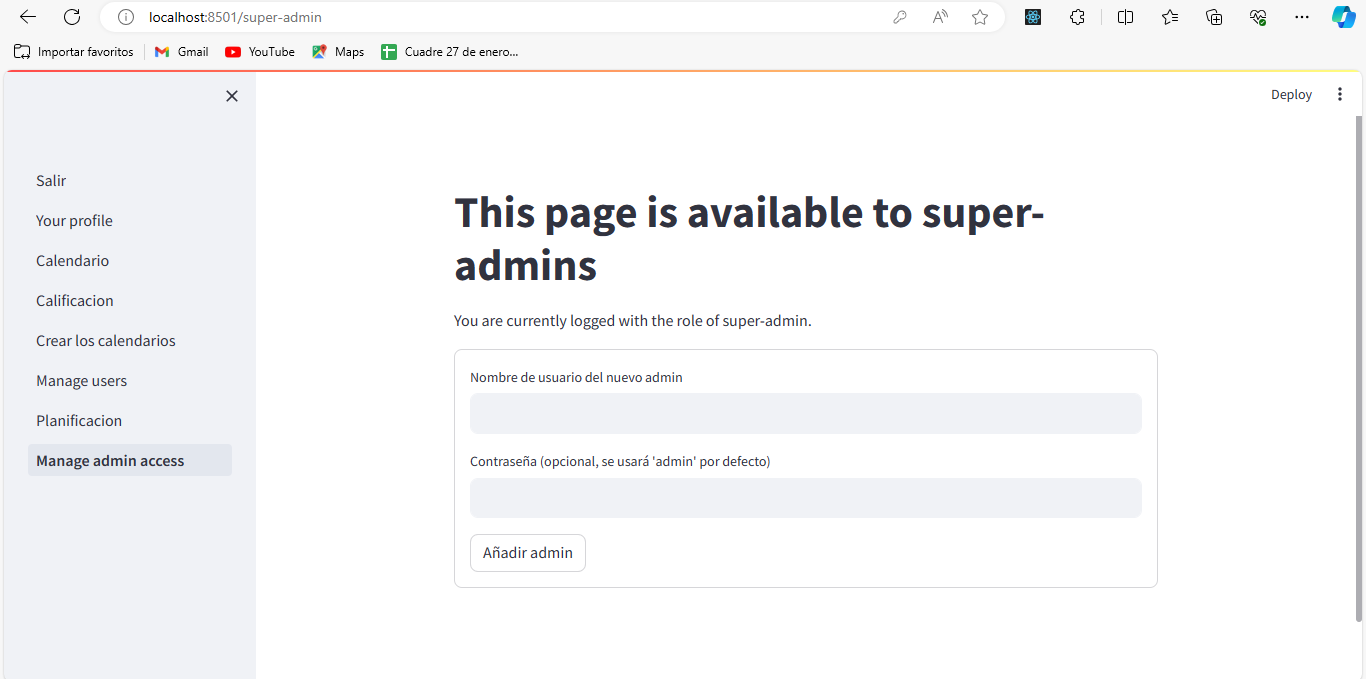
\includegraphics[width=0.5\textwidth]{gestion_acceso_admin.png} \caption{Pantalla de gestión de acceso de admin.} \end{figure} 
\subsubsection{Conclusión}

La propuesta de aplicación presentada aquí representa un avance significativo en la gestión de calendarios de exámenes, al proporcionar una solución segura y eficiente que satisface las necesidades de diferentes usuarios con diferentes niveles de acceso. Al implementar esta aplicación, las instituciones educativas pueden mejorar la experiencia de sus estudiantes y profesores, al tiempo que optimizan la planificación y distribución de los calendarios de exámenes. Se recomienda su uso para recibir retroalimentación de los usuarios y hacer las mejoras que se consideren convenientes.
\end{document}
